\chapter{Perancangan Sistem}

\section{Alur Perancangan}
\begin{figure}[h]
	\centering
	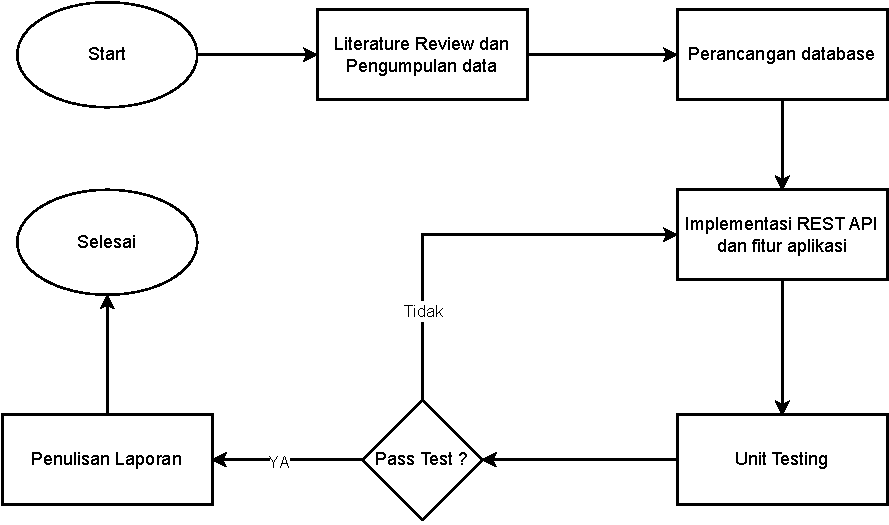
\includegraphics[width=0.75\textwidth]{drawio/alur-perancangan.drawio.pdf}
	\caption{Alur Perancangan}
	\label{alur-perancangan}
\end{figure}
Gambar \ref{alur-perancangan} menggambarkan alur perancangan sistem backend yang dibuat. Terdapat 5 tahapan dalam perancangan sistem yaitu :
\subsection{Literature Review dan Pengumpulan data}
Pada tahap ini, dilakukan pengumpulan data melalui Software Requirement Specification (SRS) yang telah dibuat oleh System Analyst (SA) serta membaca literatur ilmiah mengenai Pengembangan backend web.

\subsection{Perancangan database}
Pada tahap ini dilakukan perancangan dan implementasi ERD menggunakan Prisma sebagai framework Object Relational Mapping.

\subsection{Implementasi REST API dan fitur aplikasi}
Pada tahap ini dilakukan sesi koding untuk mengimplementasikan berbagai macam fitur aplikasi berdasarkan SRS yang telah dibuat, dan membuat API endpoint yang menghindari anti pattern.

\subsection{Unit Testing}
Pada tahap unit testing, akan dicek apakah koding udah benar dan tidak terjadi error, maka akan lanjut ke penulisan laporan. Jika kodingan masih error atau tidak lulus uji unit testing maka akan diulangi tahap Implementasi Rest dan fitur aplikasi.

\subsection{Penulisan laporan}
Pada tahap ini, akan merangkum apa saja yang dipelajari dan hasil analisis saat membuat dan mengimplementasikan software backend.

\section{Desain Sistem}
\begin{figure}[h]
	\centering
	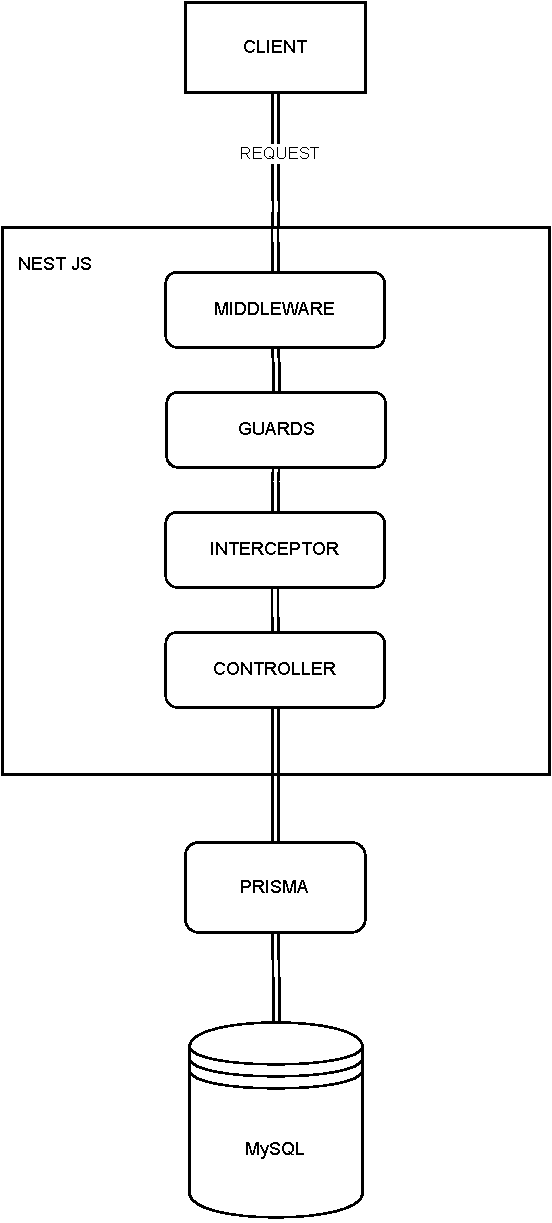
\includegraphics[width=0.35\textwidth]{drawio/sistem-desain.drawio.pdf}
	\caption{Desain Sistem}
	\label{sistem-desain}
\end{figure}
Implementasi dan perancangan RESTful API, Database, dan fungsi bisnis dikembangkan menggunakan framework NestJs. Pada NestJs terdapat beberapa komponen seperti: Middleware, Guards, Interceptor, Controller, dan Service dimana Service yang dipakai adalah Prisma untuk menghubungkan Nest ke Database System. Pada gambar \ref{sistem-desain} menjelaskan Request Lifecycle dimana gambar tersebut menjelaskan bagaiamana alur request di tangani dari awal sampai akhir.
Pada Middleware, Fungsi akan dipanggil sebelum masuk ke routing. Pada Guard, request akan dicek \textit{authenticity}, apakah request tersebut valid tidak nya. Di tahap ini juga akan dicek keamanan session menggunakan JWT dan CSRF. Setelah melalui Guard, Request akan masuk ke Interceptor dimana jika suatu request mempunyai suatu karakteristik yang ditentukan, maka akan menjalankan fungsi tambahan. Interceptor terjadi ketika request datang (pre), dan response (post). Setelah melewati Interceptor, maka function di Controller akan dijalankan, jika pada Controller tersebut perlu data dari database maka akan turun ke service Prisma untuk melakukan database call menggunakan ORM \cite{NestJS}.
